\chapter{Theoretische Grundlagen}
\label{chap:two}
\section{Bibliothek und Statistik}
\label{chap:two_one}
Die Etatplanung von Bibliotheken richtet sich nach deren Informations- und Versorgungsauftrag. Seit Beginn der 1990er Jahre kämpfen Bibliotheken mit den steigenden Preisen und der Informationsflut, zunehmenden Kommerzialisierungstendenzen in der Verlagslandschaft und neuen Medientypen. Zu nennen wären hier: die Explosion der Zeitschriftenpreise im Bereich der Science, Technology & Medicine (STM), das Aufkommen von E-Publishing und die Konzentration auf wenige Verlage Demgegenüber steigen Bibliotheksetats nur mäßig. (Moravetz, S. 161)
Um diesen Veränderungen zu begegnen, ist es wichtig, sorgsam das Bibliotheksbudget zu planen. Dies geschieht in größeren Bibliotheken durch Etatbedarfs- und Etatverteilungsmodelle. Ziel dieser Modelle ist die transparente und gerechte Verteilung knapper Ressourcen innerhalb der Bibliothek. (Moravetz, S. 172)
Grundlage auf denen diese Modelle basieren sind statistische Daten. Was sind statistische Daten? Diese Daten werden durch Evaluationsverfahren erhoben. Im bibliothekarischen Kontext sind die sammlungs-, nutzungsbezogene und die nutzerbezogene Evaluation zu finden.  Die sammlungsbezogene Evalution betrifft den Bestand, dessen Größe und Wachstum über die Jahre. Nutzungsbezogene Evalution betrifft die Lesesaalnutzung, die Ausleihe vor-Ort, die Nutzung des Fernleihservices oder Dolumentlieferdienste und die Online-Nutzung. Ziele dabei sind die Identifizierung von ausleihträchtigen Medienbeständen (Vormerkungs- und Rennerlisten), die Deacquisition schlecht oder gar nicht genutzter Titel. Ebenso kann die Evaluation von Fernleih- und Dokumentenlieferungen Hinweise auf Bestandslücken liefern. (johannsen_jochen_bestands-_2015, 255 ff). Die nutzerbezogene Evaluation ist zentriert um den Nutzer und dessen Informitionsbedürfnisse.
Fundamental ist der Unterschied zwischen den einzelnen Evaulationsverfahren in der Erhebung der Daten. Die sammlungs- und nutzungsorientierten Evaluationsverfahren basieren auf der Erhebung von quantitativen Daten wie Bestandsgröße oder der Anzahl von Ausleihen nach Titel. Während nutzerbezogene Evaluation qualitative Daten aus zum Beispiel Befragungen erhebt. (From data to decisions: using surveys, 461 ff.)

Statistriken sind wichtig…
Im deutschen Bibliothekswesen gab es den Bibliotheksindex (BIX), der ursprünglich seit 1999 für die Leistungsmessung in Öffentlichen Bibliotheken konzipiert wurde. 2002 wurde er erweitert auf Wissenschaftliche Bibliotheken. 2015 wurde der BIX aufgrund von Finanzierungsproblemen eingestellt. Daneben gibt es seit 1974 die umfangreiche Deutsche Bibliotheksstatistik (DBS). Träger der DBS sind das hbz, Kompetenznetzwerk für Bibliotheken (KBN), KMK sowie die Bibliotheken
Aufgabe dieser ist die jährliche Erhebung der Statistikdaten von Kennzahlen von Bibliotheken.  Seit 1999 werden die Daten nur noch online erfasst, ausgewertet und präsentiert. 
(https://www.egms.de/static/en/journals/mbi/2008-8/mbi000102.shtml)
Neben den Gesamtauswertungen der DBS, einer Bibliothekssuchmachine für Öffentliche Bibliotheken, bietet sie eine variable Auswertung nach individuellen Abfragen der DBS-Daten. Dennoch bietet die DBS vielmehr eine Datengrundlage für die Auswertung der Daten an.



\clearpage
Bibliotheksrahmen - Etatplanung - Etatbedarfe, Zielsetzung der Bibliothek\\
Begriffe wie Mittelallokation\\
Bestandsmanagement\\
Was ist Statistik\\
Erhebung von qualitativen und quantitativen Daten Bsp.:\\
Konzentration auf quantitative Daten wie ...\\
hat schon immer große Rolle in Bibliotheken gespielt\\
BIX, Deutsche Bibliotheksstatistik (seit wann)\\
Warum ist Messbarkeit von bibliothekarischen Daten wichtig?\\
Welchen Impact für Budgetplanung können statistische Daten haben?\\
Was können statistische Daten in Bibliotheken aussagen?\\
Welche Daten werden in Bibliotheken erhoben\\
Sammlungsbezogene Evaluierung
Nutzerbezogene Evaluation\\
Nutzungsbezogene Evaluation\\
quantitativ und qualitativ:\\
Counter-Statistiken \& Standards\\

\clearpage

\section{Datenvisualisierung}
Mit den Siegeszug des Computers in den 1980/90er Jahren sind \dots\\
Was ist unter Datenvisualisierung zu verstehen?\\
leicht verschiedene Begriffsdefinitionen
Vielzahl von Begriffen\\ 
Oberbegriff für Informationsvisualisierung / Scientific Visualization\\
Abgrenzung zu Infographics\\
Zu welchem Zweck\\
Eigenschaften\\
Wie Datenvisualisierungen gestaltet werden sollen - simpel\\
Grundlage - Daten - quantitativ / qualitativ
Warum Datenvisualisierung wichtig ist?\\
Was erzählen Datenvisualisierungen mehr als Zahlenkolonnen?\\
Perception of the eye - schnellere Auffassung
Welche Datenvisualisierungen gibt es?\\
Wo kommen Daternvisualisierungen zum Einsatz?\\



% \begin{figure}[ht]
%     \centering
%         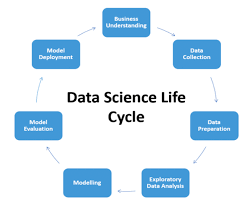
\includegraphics[width=8cm]{ds_cycle}
%         \caption{Data Science Cycle}
%         \label{fig:data science}
% \end{figure}



\clearpage
\section{Business-Intelligence-Systeme}

Was sind Business-Intelligence-Löungen?\\
Wo kommen Buisiness-Intelligence-Lösungen zum Einsatz zum Einsatz?
